\documentclass[border=0.2cm]{standalone}

% More defined colors
\usepackage[dvipsnames]{xcolor}
\usepackage{tikz,ifthen}
\usetikzlibrary{positioning}
\usepackage{xstring}
\usepackage{graphicx} %package to manage images
\usetikzlibrary{shapes.geometric}
\graphicspath{ {./images/} } 

\definecolor{green0}{RGB}{206, 222, 178}
\definecolor{green1}{RGB}{133, 194, 81}
\definecolor{blue0}{RGB}{168, 212, 228}
\definecolor{blue1}{RGB}{49, 143, 187}
\definecolor{yellow1}{RGB}{251, 189, 9}

\newcommand{\numlayerA}{8}
\newcommand{\numlayerB}{8}
\newcommand{\numlayerC}{32}
\newcommand{\numlayerD}{20}

\newcommand\stackedrectangels[9]
{
    \foreach \i [evaluate={\n=int(mod(\i,2)};] in {1,...,#1}
    {
        \node [draw, fill=#2\n, minimum width=#8cm, minimum height=#8cm] (rect#7\i)  at (#3+ \i * #5, #4 -\i * #6) {};
    }
    \node[below of=rect#7#1, align=center, node distance=2cm] {#9};
}

\begin{document}
\begin{tikzpicture}

\stackedrectangels{8}{green}{0}{0}{.4}{.4}{1}{2}{Convolution};
\stackedrectangels{8}{blue}{5}{-1}{.3}{.3}{2}{1.5}{Pooling};
\stackedrectangels{32}{green}{5}{3}{.2}{.2}{3}{1}{Convolution};
\stackedrectangels{20}{blue}{10}{1}{.2}{.2}{4}{1}{Pooling};
\node[scale = .5, left of = rect16, node distance = 10cm] (inputpic)  {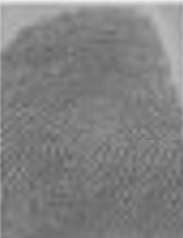
\includegraphics {images/1.3.b.input.png}};


\draw[dashed] ([xshift=-8mm, yshift=1.5cm]inputpic.south east) -- ([xshift=-8mm, yshift=1cm]inputpic.south east)-- ([xshift=-5mm, yshift=3mm] rect18.south east) -- cycle;

\draw[dashed] ([xshift=-8mm, yshift=1.5cm]rect18.south east) -- ([xshift=-8mm, yshift=1cm]rect18.south east)-- ([xshift=-5mm, yshift=3mm] rect28.south east) -- cycle;

\draw[dashed] ([xshift=-8mm, yshift=1.3cm]rect28.south east) -- ([xshift=-8mm, yshift=1cm]rect28.south east)-- ([xshift=-3mm, yshift=3mm] rect332.south east) -- cycle;

\draw[dashed] ([xshift=-4mm, yshift=8mm]rect332.south east) -- ([xshift=-4mm, yshift=5mm]rect332.south east)-- ([xshift=-3mm, yshift=3mm] rect420.south east) -- cycle;

\draw[dashed] ([xshift=-4mm, yshift=8mm]rect332.south east) -- ([xshift=-4mm, yshift=5mm]rect332.south east)-- ([xshift=-3mm, yshift=3mm] rect420.south east) -- cycle;

\draw[dashed] ([xshift=-8mm, yshift=1.3cm]rect28.south east) -- ([xshift=-8mm, yshift=1cm]rect28.south east)-- ([xshift=-3mm, yshift=3mm] rect332.south east) -- cycle;

\draw[draw = yellow1, fill = yellow1] ([xshift=2cm]rect41.north east) -- ([xshift=3cm, yshift=1mm]rect41.north east) -- ([xshift=3.3cm, yshift=5mm]rect420.south east) -- ([xshift=2.3cm, yshift=4mm] rect420.south east) -- cycle;

\draw[draw = yellow1, fill = yellow1] ([xshift=5cm]rect43.north east) -- ([xshift=6cm, yshift=1mm]rect43.north east) -- ([xshift=6.3cm, yshift=5mm]rect416.south east) -- ([xshift=5.3cm, yshift=4mm] rect416.south east) -- cycle;

\draw[draw = yellow1, fill = yellow1] ([xshift=8cm]rect44.north east) -- ([xshift=9cm, yshift=1mm]rect44.north east) -- ([xshift=9.3cm, yshift=5mm]rect411.south east) -- ([xshift=8.3cm, yshift=4mm] rect411.south east) -- cycle;

\draw[dashed] (rect44.north east) -- ([xshift=9cm, yshift=1mm]rect44.north east) -- ([xshift=9.3cm, yshift=5mm]rect411.south east) -- ([xshift=8.3cm, yshift=4mm] rect411.south east) -- cycle;


%\node[trapezium, draw = yellow1, fill = yellow1, trapezium stretches=true, trapezium angle=67.5, minimum height=7mm, right of=rect410, node distance=3cm] (t1) {}; 

%\node [draw=yellow1, rotate=42, fill=yellow1, minimum width=1cm, minimum height=5cm, right of=rect416, node distance=2.5cm] (controller1) {};

\end{tikzpicture}
\end {document}